\section{Model-Based Statistical Analysis}

\subsection{Model Selection}

\begin{table}[H]
\centering
\begin{tabular}{|l|l|l|l|l|}
\hline
& month & month + gender & month + education & month + gender + education \\
\hline
AIC & 3979.734 & 3947.393 & 3976.155 & 3946.259 \\
\hline
BIC & 3992.965 & 3965.027 & 3993.789 & 3968.293\\
\hline
\end{tabular}
\caption{Comparison of models with different covariates under the intervention group}
\label{tab:model.comp.intervention}
\end{table}

\begin{figure}[H]
\begin{subfigure}{.33\textwidth}
  \centering
  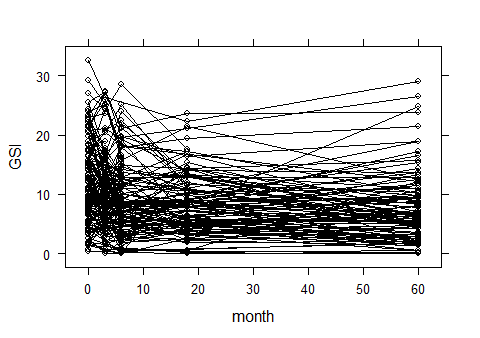
\includegraphics[width=1\linewidth]{../../plots/trellis_treatment.png}
  \caption{trellis plot of all subjects in the intervention group}
\end{subfigure}
\begin{subfigure}{.33\textwidth}
  \centering
  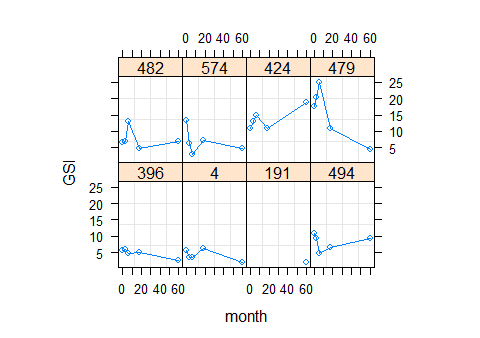
\includegraphics[width=1\linewidth]{../../plots/trellis_subset_treatment.png}
  \caption{trellis plot of randomly selected subjects}
\end{subfigure}
\begin{subfigure}{.33\textwidth}
  \centering
  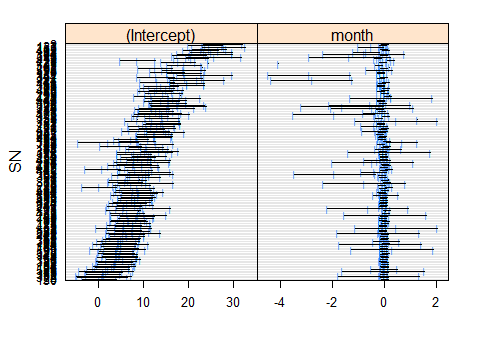
\includegraphics[width=1\linewidth]{../../plots/interval_treatment.png}
  \caption{confidence intervals of parameters from individual linear models}
\end{subfigure}
\caption{Diagnostic plots for selection of random effects for the intervention group}
\label{fig:diagnostic.treatment}
\end{figure}

\begin{table}[H]
\begin{minipage}{0.5\textwidth}
\centering
\resizebox{\linewidth}{!}{
\begin{tabular}{|l|l|l|l|}
\hline
& no mixed effect & intercept & intercept and slope \\
\hline
AIC & 3946.259 & 3646.267 & 3643.133 \\
\hline
BIC & 3968.293 & 3672.708 & 3678.388 \\
\hline
\end{tabular}
}
\caption{Comparison of models with different mixed effects under the intervention group}
\label{tab:model.comp.treatmemt.me}
\end{minipage}
\hfill
\begin{minipage}{0.5\textwidth}
\centering
\resizebox{\linewidth}{!}{
\begin{tabular}{|l|l|l|l|}
\hline
& no mixed effect & intercept & intercept and slope \\
\hline
no mixed effect & N/A & 0 & 0 \\
\hline
intercept & 0 & N/A & 0.028 \\
\hline
intercept and slope & 0 & 0.028 & N/A \\
\hline
\end{tabular}
}
\caption{P values of Likelihood Ratio tests between models with different mixed effects under the intervention group}
\label{tab:model.comp.treatment.me.lrt}
\end{minipage}
\end{table}

\subsection{Change in Mental Distress over Time in Each Group}

\subsubsection{Assumption Check}

\begin{figure}[H]
\begin{subfigure}{.5\textwidth}
  \centering
  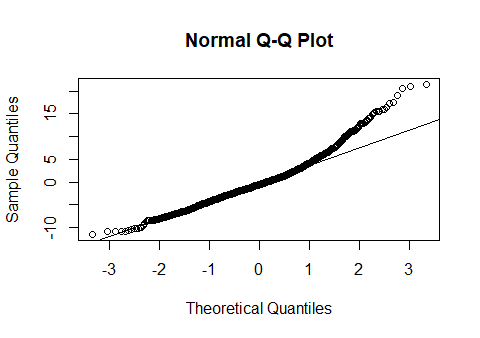
\includegraphics[width=1\linewidth]{../../plots/qq_residual_treatment.png}
  \caption{residual QQ plot}
\end{subfigure}
\begin{subfigure}{.5\textwidth}
  \centering
  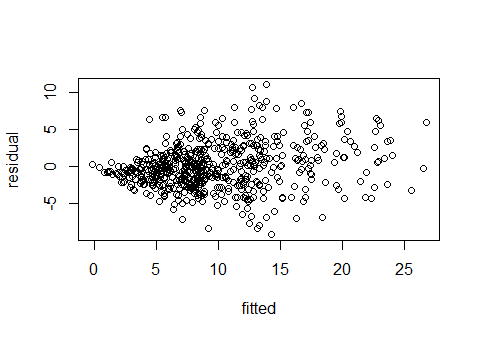
\includegraphics[width=1\linewidth]{../../plots/residual_treatment.png}
  \caption{fitted value vs. residual (t-test: 1, Wilcoxon: 0.204)}
\end{subfigure}
\caption{Visualizing the residuals of the LME model under the intervention group}
\label{fig:residual.treatment}
\end{figure}

\begin{figure}[H]
\begin{subfigure}{.5\textwidth}
  \centering
  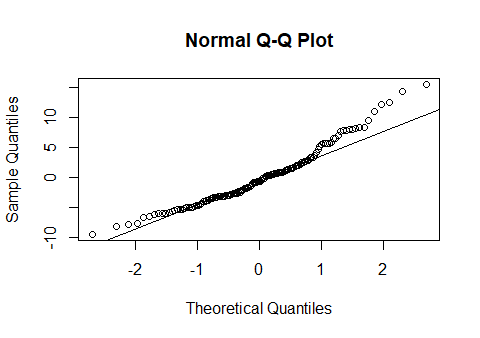
\includegraphics[width=1\linewidth]{../../plots/qq_intercept_treatment.png}
  \caption{QQ plot for the random effects on the intercept (t-test: 1, Wilcoxon: 0.335)}
\end{subfigure}
\begin{subfigure}{.5\textwidth}
  \centering
  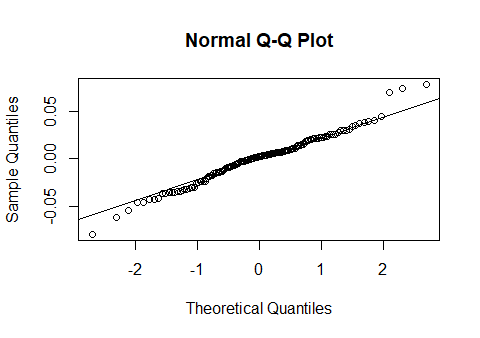
\includegraphics[width=1\linewidth]{../../plots/qq_slope_treatment.png}
  \caption{QQ plot for the random effects on the slope (t-test: 1, Wilcoxon: 0.781)}
\end{subfigure}
\caption{Visualizing the random effects under the intervention group}
\label{fig:re.treatment}
\end{figure}

\subsubsection{Linear Mixed Model}

\subsubsection{Generalized Estimating Equation}

\begin{table}[H]
\begin{minipage}{0.5\textwidth}
\centering
\resizebox{\linewidth}{!}{
\begin{tabular}{|l|r|r|r|r|r|}
\hline
  & Value & Std.Error & DF & t-value & p-value\\
\hline
(Intercept) & 11.933 & 2.758 & 465 & 4.326 & 0.000\\
\hline
month & -0.047 & 0.008 & 465 & -5.671 & 0.000\\
\hline
gender2 & 2.764 & 0.925 & 141 & 2.990 & 0.003\\
\hline
education & -0.249 & 0.190 & 141 & -1.314 & 0.191\\
\hline
\end{tabular}
}
\caption{Output of Linear Mixed Model under the intervention group}
\label{tab:lme.treatment}
\end{minipage}
\hfill
\begin{minipage}{0.5\textwidth}
\centering
\resizebox{\linewidth}{!}{
\begin{tabular}{|l|r|r|r|r|r|}
\hline
  & Estimate & Naive S.E. & Naive z & Robust S.E. & Robust z\\
\hline
(Intercept) & 11.162 & 2.484 & 4.494 & 2.538 & 4.397\\
\hline
month & -0.047 & 0.010 & -4.477 & 0.008 & -5.852\\
\hline
gender2 & 2.827 & 0.834 & 3.391 & 0.869 & 3.253\\
\hline
education & -0.194 & 0.170 & -1.146 & 0.173 & -1.125\\
\hline
\end{tabular}
}
\caption{Output of GEE model under the intervention group}
\label{tab:gee.treatment}
\end{minipage}
\end{table}

\subsection{Effectiveness of Intervention}

\subsubsection{Linear Mixed Model}

\subsubsection{Assumption Check}

\subsubsection{Generalized Estimating Equation}

\subsection{Handling Missing Data}

\subsubsection{Change in Mental Distress over Time in Each Group}

\subsubsection{Effectiveness of Intervention}
